\chapter{Data Preparation}

	\section{Data processing and data wrangling}
	
    Data preparation is the process of transforming the acquired dataset into a dataset which can be fed into learning algorithms and is cleaned of impurities in such a way, that the learning results are likely satisfactory. Impurities may be missing values, shifted columns, encoding errors or different data formats. 
    Data preparation includes data wrangling, data cleaning, and feature extraction. What is left should be a uniform dataset, which is in a format that is understandable by the desired algorithms.
    
        \subsection{Alternatives}
        The chosen dataset consists of files in \ac{JSON}. Several alternatives for storage and transforming the data exist. 
        
        \paragraph{Storage Location}
        Within the constraints of the thesis, three options are available for data storage. Firstly, data can be stored locally on the available machine. The data is available without internet access, and the local machine has high read/write speeds. This option requires no additional learning, and is free of charge for the department. A multitude of libraries exist for accessing files on a local filesystem. A downside is the limited scalability in terms of storage capacity and read/write operations. Additionally, local storage makes the data only available to this specific machine.
        
        Storing data on a cloud filesharing system is easy to operate and free of usage-bound charges. The storage space is virtually unlimited. Accessing files on sharing platforms is feasible but tedious. The access can be shared within the company context, but everyone is subject to the limited accessibility. Using a files storage service could be of use for transferring data without a physical connection. Still, this is the only recommended use case in this context.
        
        The third option is storing the data using a specialized storage service, such as AWS S3. While the learning overhead is higher in the beginning, the scalability is a convincing argument. Billing is according to usage, but adequate because of the high connectivity with other cloud-based ML service offerings inside and outside of SAP.
        
        \begin{table}[ht]
            \centering
            \caption{Comparison of available Storage Options}
            \begin{tabular}{c|lll}
                \toprule
                &\textbf{Local} & \textbf{Cloud Filesharing} & \textbf{Specialized Storage Services} \\
                \midrule
                \vspace{0.5cm}
                Example     & \begin{tabular}[c]{@{}l@{}}2.6GHz \\ 512GB SSD\end{tabular} & Microsoft OneDrive                                                        & AWS S3                                                                                                 \\
                \vspace{0.5cm}
                Ease of use & high                                                        & high                                                                      & higher learning overhead                                                                               \\
                \vspace{0.5cm}
                Cost        & free of charge                                              & free of charge                                                            & \begin{tabular}[c]{@{}l@{}}billing according to \\ used storage space\end{tabular}                     \\
                \vspace{0.5cm}
                Scalability & limited                                                     & unlimited                                                                 & unlimited                                                                                              \\
                \vspace{0.5cm}
                Data access & local                                                       & \begin{tabular}[c]{@{}l@{}}limited remote \\ access capacity\end{tabular} & \begin{tabular}[c]{@{}l@{}}local, remote, high \\ connectivity to \\ ML service offerings\end{tabular}
                
            \end{tabular}
            \label{tabelle:storage}
        \end{table}
        
        \paragraph{Data Format}
        The data is still available only in the from \ac{JSON} documents.
        
        - transforming json documents into dataframe rows
        
    \subsection{Theoretical Implementation}
    For the data wrangling the invoices have to be read into memory and then processed into a reusable structure. Each document will be read into memory, then the necessary information will be extracted. All invoices will be combined into one data structure, which then is persisted for later use.

    \begin{figure}[ht]
        \centering
        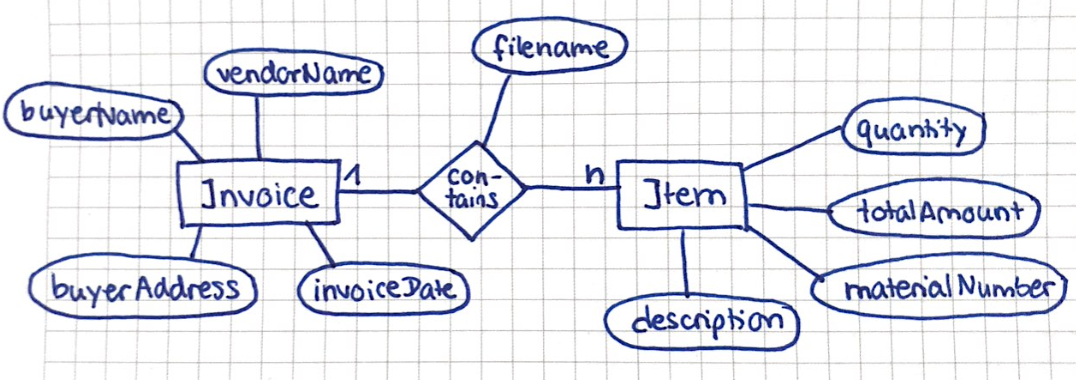
\includegraphics[height=5cm]{Bilder/practical/entity_relationship.png}
        \caption{Entity Relationship Diagram for Invoce Documents}
        \label{fig:er}
    \end{figure}

	The data for an invoice and its contained items is stored in an array of objects. This is also shown in code example (\ref{code:JSONSchema}) of a shortened JSON Schema for one invoice. The array "annotations" contains objects. One object represents information such as the invoice date or the unit price. 
	Information about invoice items have labels containing the prefix "lineItem". One invoice containing several items is represented by duplicate values of one label (in the example \ref{code:JSONInvoice} the label "lineItem.description.value"). Here, the order of the labels has to be retained during data wrangling to ensure not mixing up information about different invoice items.

	\lstinputlisting[
	label=code:JSONInvoice,    % Label; genutzt für Referenzen auf dieses Code-Beispiel
	caption=JSON of one invoice,
	captionpos=b,               % Position, an der die Caption angezeigt wird t(op) oder b(ottom)
	style=EigenerPythonStyle,   % Eigener Style der vor dem Dokument festgelegt wurde
	firstline=0,                % Zeilennummer im Dokument welche als erste angezeigt wird
	lastline=23                 % Letzte Zeile welche ins LaTeX Dokument übernommen wird
	]{Quellcode/invoice.json}
	
    \subsection{Practical Implementation}

	The files are processed in python, using the library "json". Each file is opened, and decoded with python's build in json decoder. The hierarchy is traversed until the array "annotations" is reached. Now, the tuples of label and text are saved. This process is split up into invoice and item labels.
	
	The information on invoices is stored in a tabular data structure, a python pandas DataFrame. Worth mentioning is that some invoices contain more information than others. In this case, invoices are still appended into one table, but fields for non-existent values are left empty. The filename is the unique identificator for one invoice.
	
	\begin{figure}[ht]
		\centering
		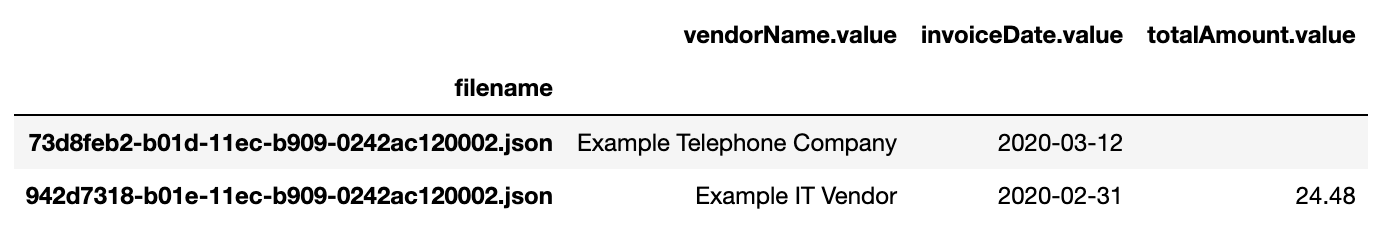
\includegraphics[height=2.5cm]{Bilder/practical/df_invoices.png}
		\caption{Exemplary depiction for processed invoices in a DataFrame}
		\label{fig:df-invoices}
	\end{figure}

	Similarly, information on the invoice items is retrieved from the documents and stored in a pandas DataFrame. Every invoice item has an unique id and can be linked to the respective invoice through the filename.
	
	\begin{figure}[ht]
		\centering
		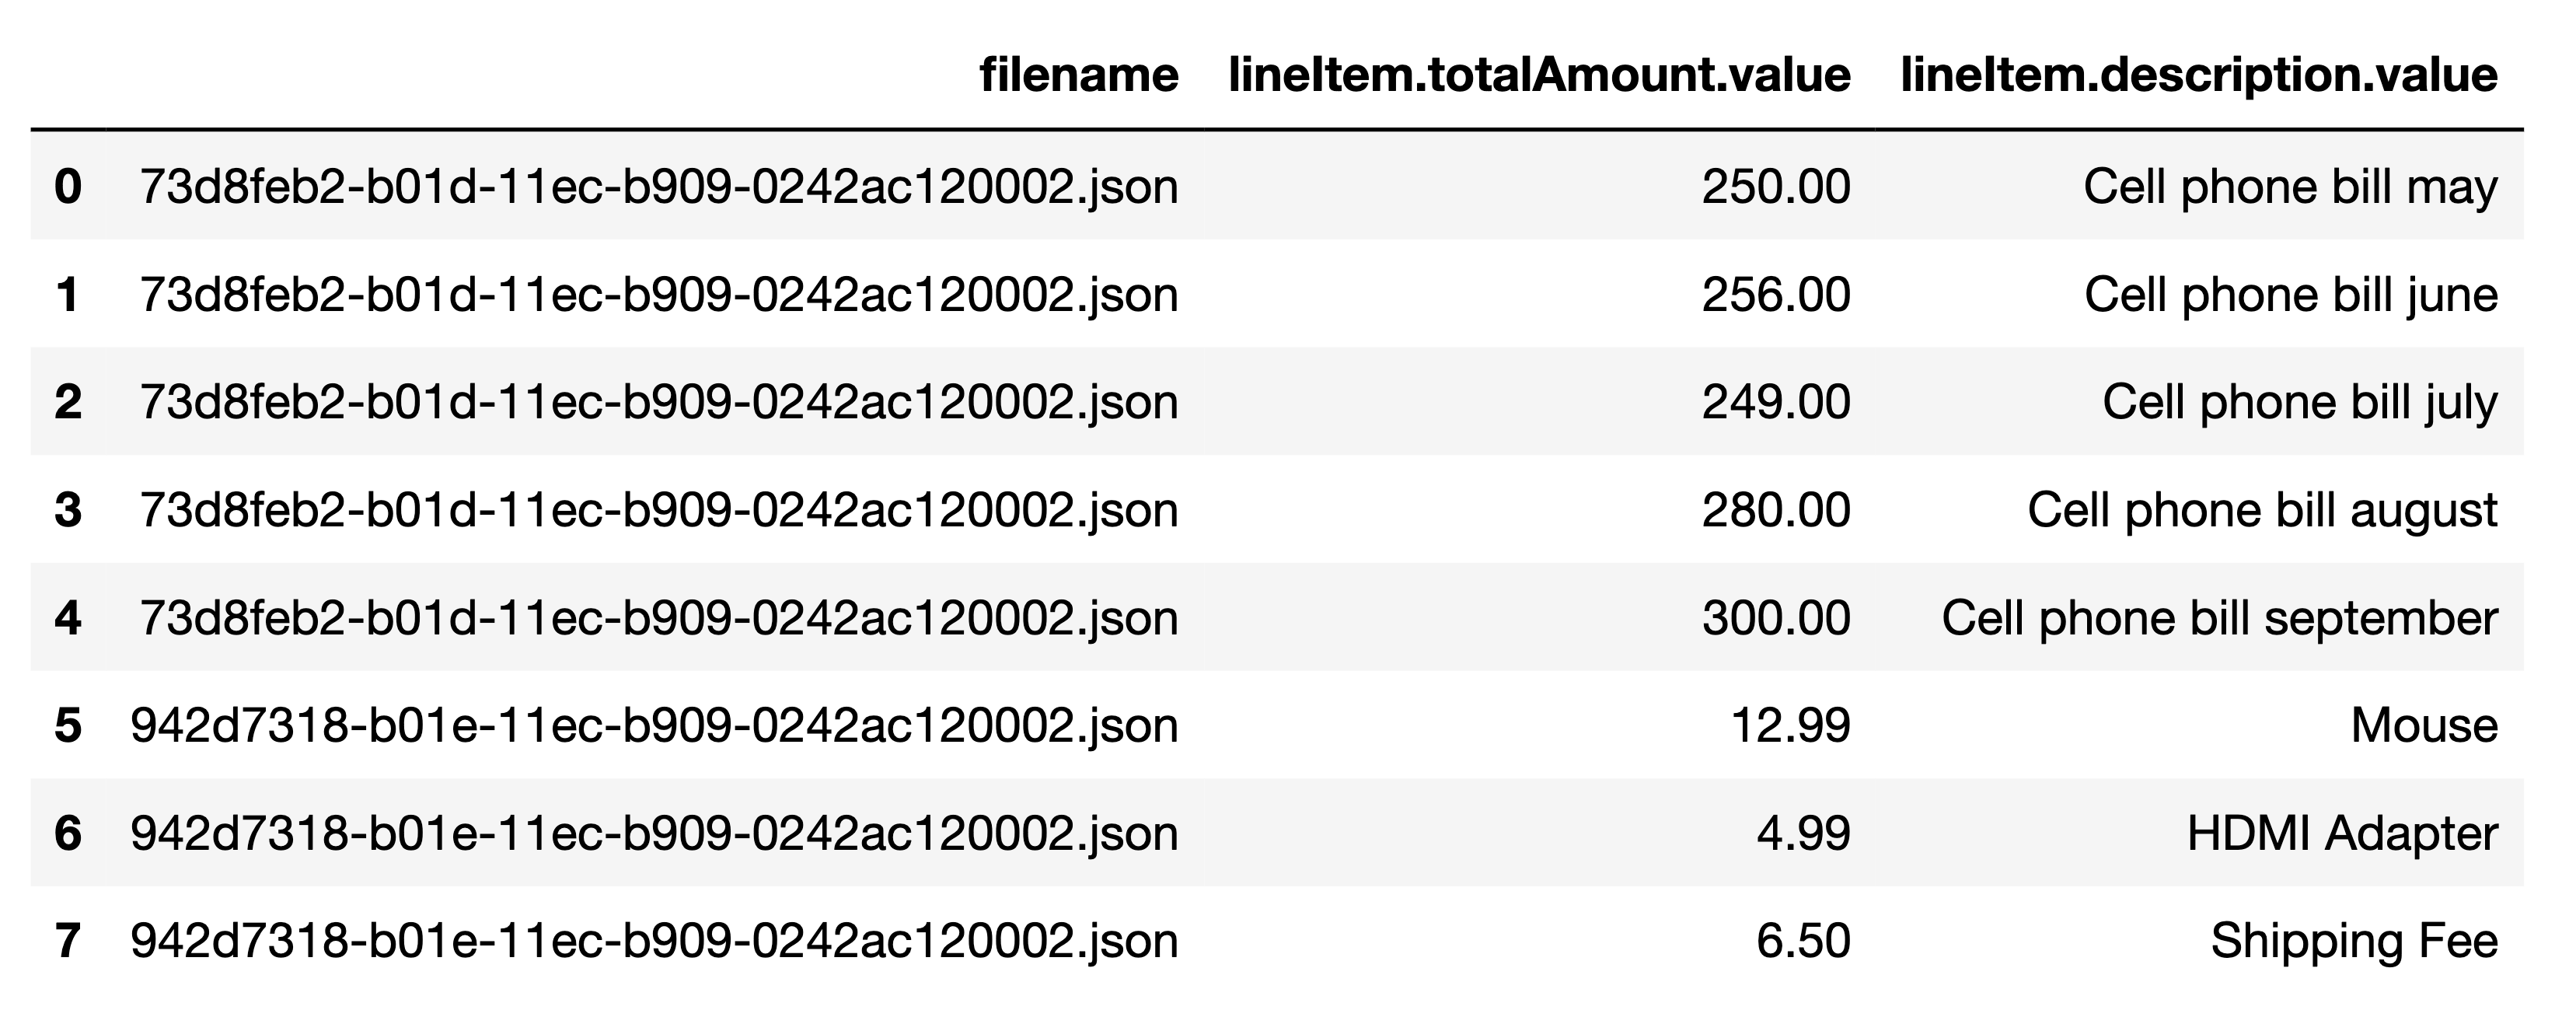
\includegraphics[height=6cm]{Bilder/practical/df_lineitems.png}
		\caption{Exemplary depiction for processed invoice items in a DataFrame}
		\label{fig:df-invoices}
	\end{figure}
	
	The resulting two DataFrames are serialized with the python standard library "pickle".  The data can be efficiently loaded into memory and reserialized again with this library.
	
	This processing step allowed for storing the initial 5.12GB of data in a more usable format and takes up only a total of 393MB. Even further improvements to storage will be dicussed later on.

	The process of reading files from the disk is not inherently an expensive one, but in the realms of many thousand documents, processing times soon reach several days. Observing the execution of the python code showed a peculiarity: While the utilization of the used processor was consequently at the maximum, only one process is executed, leaving the total CPU usage at only 20\%. 
	
	\begin{figure}[ht]
		\centering
		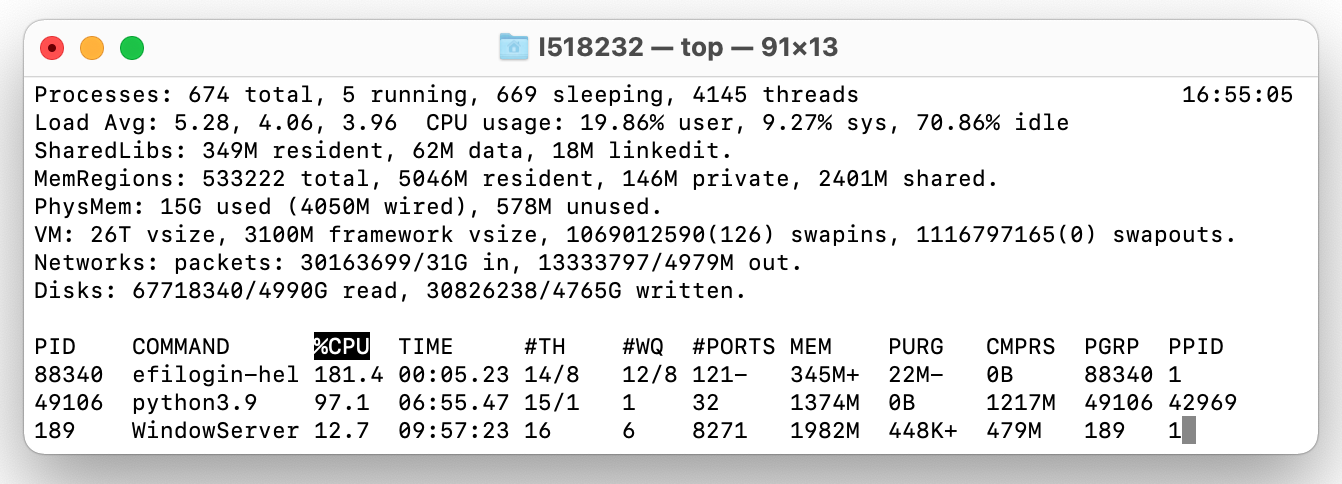
\includegraphics[height=4cm]{Bilder/practical/python_processes.png}
		\caption{Exemplary depiction for processed invoice items in a DataFrame}
		\label{fig:df-invoices}
	\end{figure}
	
	
	One question that may now arise is: Why doesn't python split up the workload and employ the full capacity of the machine?
	This can be explained with the design of the Python interpreter. The \ac{GIL} controls access to the Python Virtual Machine executing the code. This lock only allows exactly one thread to run at a time \cite{corePython}. This of course is not favorable, as valuable CPU capacity is unused. Fortunately, the \ac{GIL} behaves in a special way regarding C code, and I/O operations in Python utilize C code: the lock is released before executing a C routine \cite{corePython}. This allows to bypass the (in this case) inconvenient locking mechanism. 
	
	Different python libraries exploit this speciality and allow to spawn a pool of different processes, which then execute calls asynchronously. One example is the ProcessPoolExecutor. A notable restriction is that only picklable objects can be submitted for multiprocessing. This concerns both fuction and its parameters. While this is not a problem in this task, this restriction will become important later on in the section about feature extraction.
	


	
	\section{Data cleaning}
    - removing stopwords from several languages
        
    - removing numbers and interpunction
    
    - tokenization
	The task of data cleaning was also completed using python scripts. The library \ac{NLTK}
	
	\begin{lstlisting}[language=sh]
$ python3 -c 'import cleaner; print(cleaner.clean("500grams of special baking flour type 504"))' 
>>>  ['of', 'special', 'baking', 'flour', 'type']
	\end{lstlisting}
	 
	\section{Considerations of Space and Time Complexity}
	The dataset consists of over 150.000 invoices, and in those invoices, over 350.000 items are listed. 
	With hardware-limitation in place, an optimized approach for storing and processing the data is required. 
	Several considerations for speeding up processing time and reducing storage space can be made. 
	In the following, the observations are explained and approaches for improvement are given.

		\subsubsection{Duplicates and space complexity}
		Investigation shows, there are only 79.741 unique descriptions for the listed items. By saving only the unique values, the required space is reduced to less than one fourth compared to before. Additionally, this step is required by most machine learning models, as duplicate input values can skew the outcome. The model is chosen later, so this processing step leaves the model selection more open to different kinds of learning algorithms.
		
		\subsubsection{Reconstructing Relationships and time complexity of searching}
		After the deletion of duplicate descriptions (documents in the corpus), the 
		
		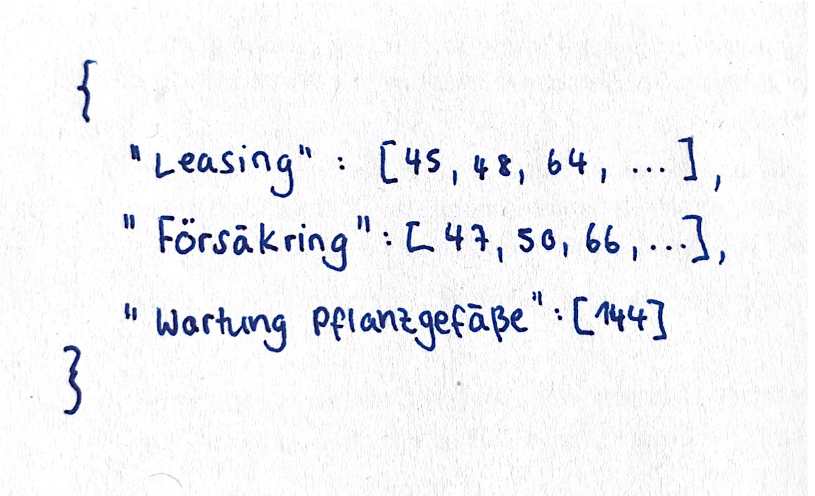
\includegraphics[height=8cm]{Bilder/description_map.png}

Explain how I want to store the data. Explain the successive artifacts.

        
        \section{Feature Extraction and Feature Engineering}
        The majority of pupular ML algorithms require the input of scalar, vector or matrix data. A form of ML models, which work with textual input will be discussed later in this section. 
        But since many algorithms were not designed to work with textual data, a transformation is required before already existing algorithms can be applied. Several methods for representing text as mathematical object will be discussed in the following.
    
            \subsection{Alternatives}
            \subsubsection{One-hot encoding}
            
    
            \subsubsection{Bag of Words Model}
            Following three documents will be considered to explain the workings of the \ac{BoW} model:
    
            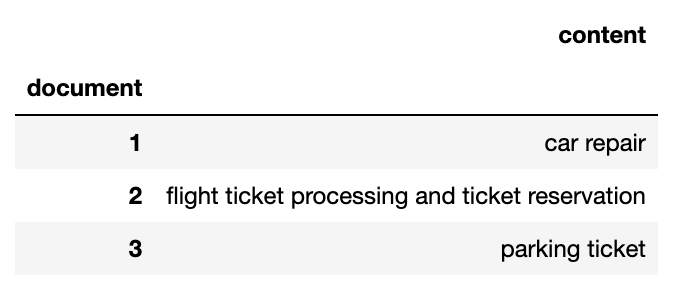
\includegraphics[height=3cm]{Bilder/corpus_bow.png}
            
            A corpus is transformed into the \ac{BoW} representation in two steps. 
            
            Firstly, the vocabulary is determined. 
            The vocabulary is a collection of all words occuring in the corpus. Every word is contained exactly once, regardless of the actual number of occurrences. The vector represenation of one document is of the same length as the vocabulary. One document being represented by one vector, a corpus of several documents can be represented as a matrix. The resulting matrix has the size $ |D|*|V| $, with $|D|$ being the number of documents in the corpus, and $|V|$ being the size of the vocabulary.
            
            Secondly, for each combination of one document $ d_{i} $ and one word $ v_{j} $ in the vocabulary, the occurrences are counted. The times, how often the specific word is contained in the document is noted in the matrix at location$  ij $.
            
            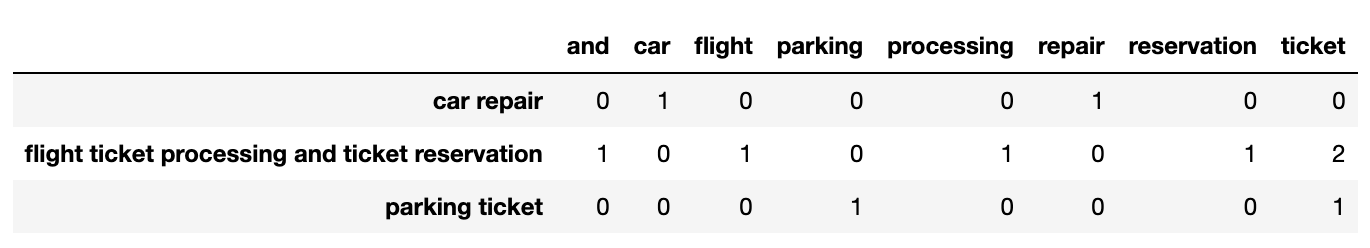
\includegraphics[height=2.9cm]{Bilder/bow.png}
    
            The result of vectorization are three vectors:
            \[ d_{1} = [0,1,0,0,0,1,0,0] \]
            \[ d_{2} = [1,0,1,0,1,0,1,2] \]	
            \[ d_{3} = [0,0,0,1,0,0,0,1]\]
    
    
            This vectorization method can be implemented with ease and in a computationally efficient manner. The \ac{BoW} model allows for a very intuitive understanding of documents, since texts consisting of the same words are considered topically related. 
            
            One of the drawbacks of this method is that no consideration is paid to words being repeated in one document. Additionally, no semantic relationship between words or documents can be inferred. 
            Further, it can be stated, that the \ac{BoW} representation fails to capture the meaning of synonyms. This becomes obvious with an example: document $ d_{1} $ and $ d_{3}$ would be considered to belong into the topic of transportation or automotives. The \ac{BoW} representation suggests topical proximity between document $ d_{2} $ and $ d_{3}$ , through the shared word "ticket". "Ticket" here is used in both the meaning of an entrace pass ($d_{2}$) and in the meaning of a note for a traffic offence  ($d_{3}$). 
            
            To conclude, the \ac{BoW} model is a straightforward text representation method. Still, it fails to capture several aspects of the natural language.
            
            \subsubsection{Tf-Idf}
            The \ac{TF-IDF} model aims to capture more meaning from the corpus by considering the composition of the whole corpus for the calculation of individual document vectors.
            
            \ac{TF-IDF} makes two assumptions about natural language:
            
            \subparagraph{1 Term Frequency}
            
            A word $t_{i} $ which occurs very frequently in one document is considered to describe a text very well. The occurences of one word in one document is denoted as $ \#( t_{i}) $.
            One additional consideration needs to be made regarding the document length. In a document of length $ |d_{2}| = 6 $ and a document of length  $ |d_{3}| = 2 $, the word $ t_{i} $occuring once would be considered equally important to each document. Of course, the word should be considered more important to $ d_{3} $, since it accounts for a larger share of the text. The measure resulting from both ideas is the term frequency:
            
            \[ TF(t_{i}, d_{j}) =   \dfrac{\#( t_{i})}{|d_{j}|} = \dfrac{occurences \; of \; word \; t_{i} \: in \; document \;\:   d_{j}}{legth \; of \; d_{j}} \]
            
            \subparagraph{2 Inverse Document Frequency}
            A word $t_{i} $ which occurs in a large number of documents does not describe one document well. Words occuring in many documents often are articles or pronouns (stopwords) which do not provide value when inspecting the content of a text. The inverse document frequence is a measure accounting for this fact. The inverse document frequency of a word is the proportion between the number of documents in the corpus and the number of documents containing the word. The logarithm is applied, as the importance of a word does not increase proportionally to the number of occurrences.
        
            
            \[ TF(t_{i}, d_{j}) = \log \dfrac{|D|}{\#(d_{t_{i}}) } =  \log \dfrac{number \;  of\;  documents \;  in \; corpus \; D}{ number \; of \; documents \; containing \; word \; t_{i}} \]
            
            Combining both assumptions, the \ac{TF-IDF} measure is created:
            
            \[ TFIDF(t_{i}, d_{j}) \;=\; TF(t_{i}, d_{j}) * TF(t_{i}, d_{j})\]
            
            For the corpus displayed in the previous section the document vectors calculated with the \ac{TF-IDF} measure are:
            
                    
            \begin{align}
                &d_1 = & [ 0\;	&0.707107\;	0\;	0\;	0\;	0.707107\;	0\;	0 \\
                &d_2 = & [ 0.39798\;	&0\;	0.39798\;	0\;	0.39798	0\;	0.39798	0.605349 
            \end{align}
                
                \[d_1 = \begin{bmatrix} 0\;	0.707107\;	0\;	0\;	0\;	0.707107\;	0\;	0 \end{bmatrix}	 \\
                d_2 =  \;\begin{bmatrix} 0.39798\;	0\;	0.39798\;	0\;	0.39798	0\;	0.39798	0.605349 \end{bmatrix} \\
                d_3 = \;\begin{bmatrix} 0\;	0\;	0\;	0.795961	0\;	0\;	0\;	0.605349 \end{bmatrix} \]
                
            The \ac{TF-IDF} measure corrects some of the pitfalls of the \ac{BoW} model. It certainly is less vulnerable to skewing by stopwords as words are ranked by importance to each document and the all over corpus. 
            
            Just as the \ac{BoW} representation, \ac{TF-IDF} suffers from high-dimensionality. The vectors contain one element for each word in the vocabulary, resulting in vectors which are inefficient to handle.
            Also, \ac{TF-IDF} fails to represent the topical relationship between $ d_{1} $ and $ d_{3}$. 
            
            \subsubsection{Word Embeddings}
             Again, the most desirable vector representation consists of dense low-dimensional vectors which are close to each other if the words are considered similar. The lack of "understanding" of related words, and the problem of high-dimensionality is corrected with the third presented option: Word Embeddings.
            
            An embedding is a translation of a word into a high-quality vector. The model does so, as it has been trained on a large set of natural language data. Popular embeddings include word2vec, fasttext and doc2vec. Word2Vec is the original model and will be discussed in the following. 
            
            The word2vec model assumes that words appearing in a similar context are also similar to each other. There are two options for the input and output: the word $w_i$ and its context $c_i$.
            
            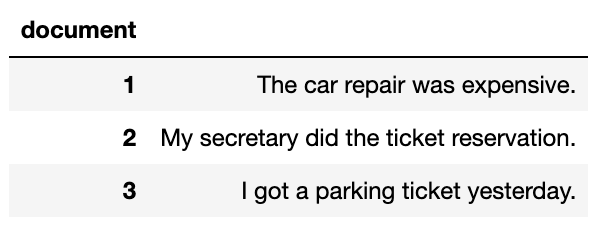
\includegraphics[height=4cm]{Bilder/word2vec/documents.png}
            
            \subparagraph{\aclu{CBOW}} 
            With the \ac{CBOW} architecture the word2vec model is trained to predict a word using the context as input. A sliding window of a predefined size is moved along the text. 
            
            \begin{figure}[ht]
                \centering
                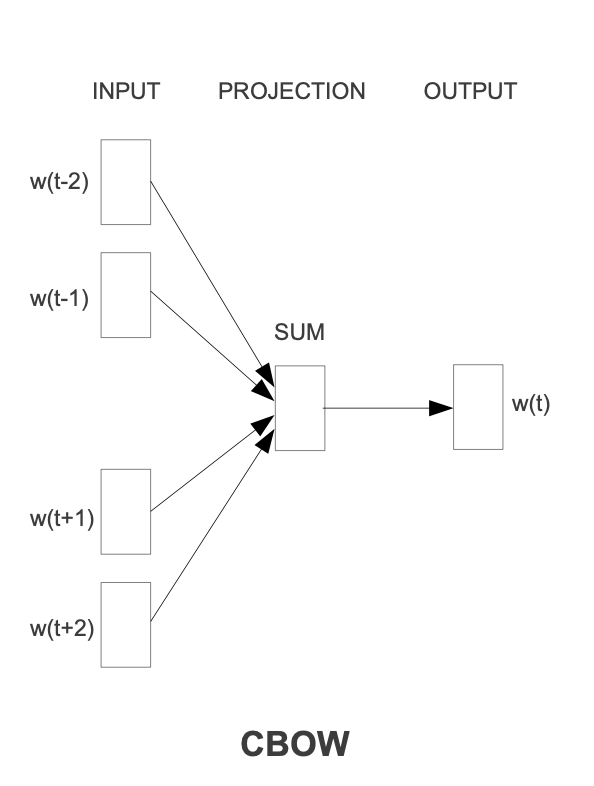
\includegraphics[height=6cm]{Bilder/word2vec/architecture_cbow.png}
                \caption{\aclu{CBOW} architecture\\\ with sliding window of size $C=5$ }
                \label{fig:cbow-architecture}
            \end{figure}
        
            \subparagraph{Skipgram} 
            With the skipgram architecture the word2vec model is trained to predict the context of the input word.
            
            \begin{figure}[ht]
                \centering
                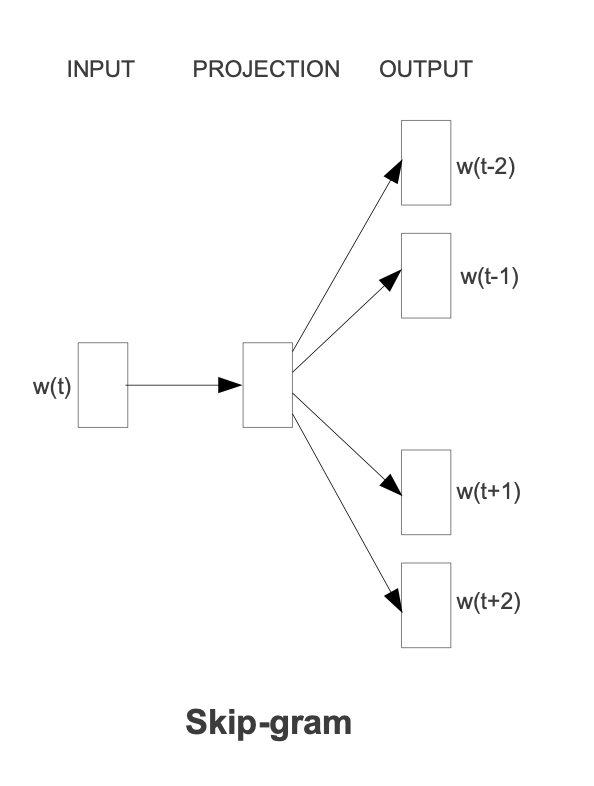
\includegraphics[height=6cm]{Bilder/word2vec/architecture_skipgram.png}
                \caption{Skipgram architecture\\\ with sliding window of size $C=5$ }
                \label{fig:cbow-architecture}
            \end{figure}
        
            \begin{figure}[ht]
                \centering
                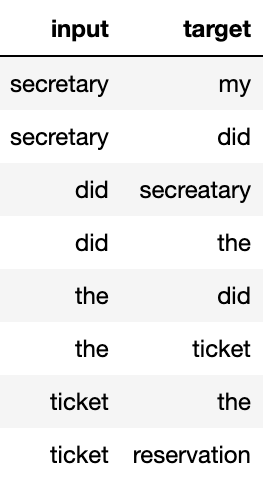
\includegraphics[height=8cm]{Bilder/word2vec/skipgram.png}
                \caption{Observations for training with skipgram architecture}
                \label{fig:cbow-architecture}
            \end{figure}
            
            
            \subparagraph{Negative Sampling}
            
            
            Word2Vec uses either SKIPGram or CBOW.
            
            Word2vec can utilize two models for selecting observations: either skipgram or \ac{CBOW}. 
            
            \subsection{Theoretical Implementation}
            
            \subsection{Practical Implementation}
            Tf-Idf weighed USEM Word vectors